% Meta-PID Network Architecture - PlotNeuralNet Style
% 需要安装: pdflatex + tikz
% 编译: pdflatex meta_pid_network_architecture.tex

\documentclass[border=8pt, multi, tikz]{standalone}
\usepackage{import}
\usepackage{tikz}
\usepackage{amsmath}
\usepackage{amsfonts}
\usepackage{amssymb}
\usepackage{bm}

\usetikzlibrary{positioning, shapes.geometric, arrows.meta, calc, shadows, 3d, decorations.pathreplacing}

% 定义颜色(Nature/Science风格)
\definecolor{inputcolor}{RGB}{52, 152, 219}      % 蓝色
\definecolor{encodercolor}{RGB}{231, 76, 60}     % 红色
\definecolor{hiddencolor}{RGB}{243, 156, 18}     % 橙色
\definecolor{outputcolor}{RGB}{39, 174, 96}      % 绿色
\definecolor{activationcolor}{RGB}{155, 89, 182} % 紫色
\definecolor{textcolor}{RGB}{44, 62, 80}         % 深灰

% 定义3D立方体绘制命令(带垂直渐变:上浅下深)
\newcommand{\drawcube}[6]{
    % #1: x position
    % #2: y position  
    % #3: width
    % #4: height
    % #5: depth
    % #6: color
    
    \coordinate (A) at (#1, #2);
    \coordinate (B) at ($(A) + (#3, 0)$);
    \coordinate (C) at ($(B) + (0, #4)$);
    \coordinate (D) at ($(A) + (0, #4)$);
    
    \coordinate (E) at ($(A) + (#5*0.3, #5*0.3)$);
    \coordinate (F) at ($(B) + (#5*0.3, #5*0.3)$);
    \coordinate (G) at ($(C) + (#5*0.3, #5*0.3)$);
    \coordinate (H) at ($(D) + (#5*0.3, #5*0.3)$);
    
    % 绘制后面的面(较暗,带渐变)
    \fill[top color=#6!70, bottom color=#6!90, opacity=0.8] (E) -- (F) -- (G) -- (H) -- cycle;
    \fill[left color=#6!75, right color=#6!95, opacity=0.8] (D) -- (H) -- (G) -- (C) -- cycle;
    
    % 绘制前面的面(主面,上浅下深渐变)
    \fill[top color=#6!50, bottom color=#6!100, opacity=0.95] (A) -- (B) -- (C) -- (D) -- cycle;
    \fill[left color=#6!75, right color=#6!100, opacity=0.85] (B) -- (F) -- (G) -- (C) -- cycle;
    \fill[top color=#6!65, bottom color=#6!90, opacity=0.8] (E) -- (F) -- (B) -- (A) -- cycle;
    
    % 绘制边框
    \draw[black, thick] (A) -- (B) -- (C) -- (D) -- cycle;
    \draw[black, thick] (E) -- (F) -- (G) -- (H) -- cycle;
    \draw[black, thick] (A) -- (E);
    \draw[black, thick] (B) -- (F);
    \draw[black, thick] (C) -- (G);
    \draw[black, thick] (D) -- (H);
}

\begin{document}
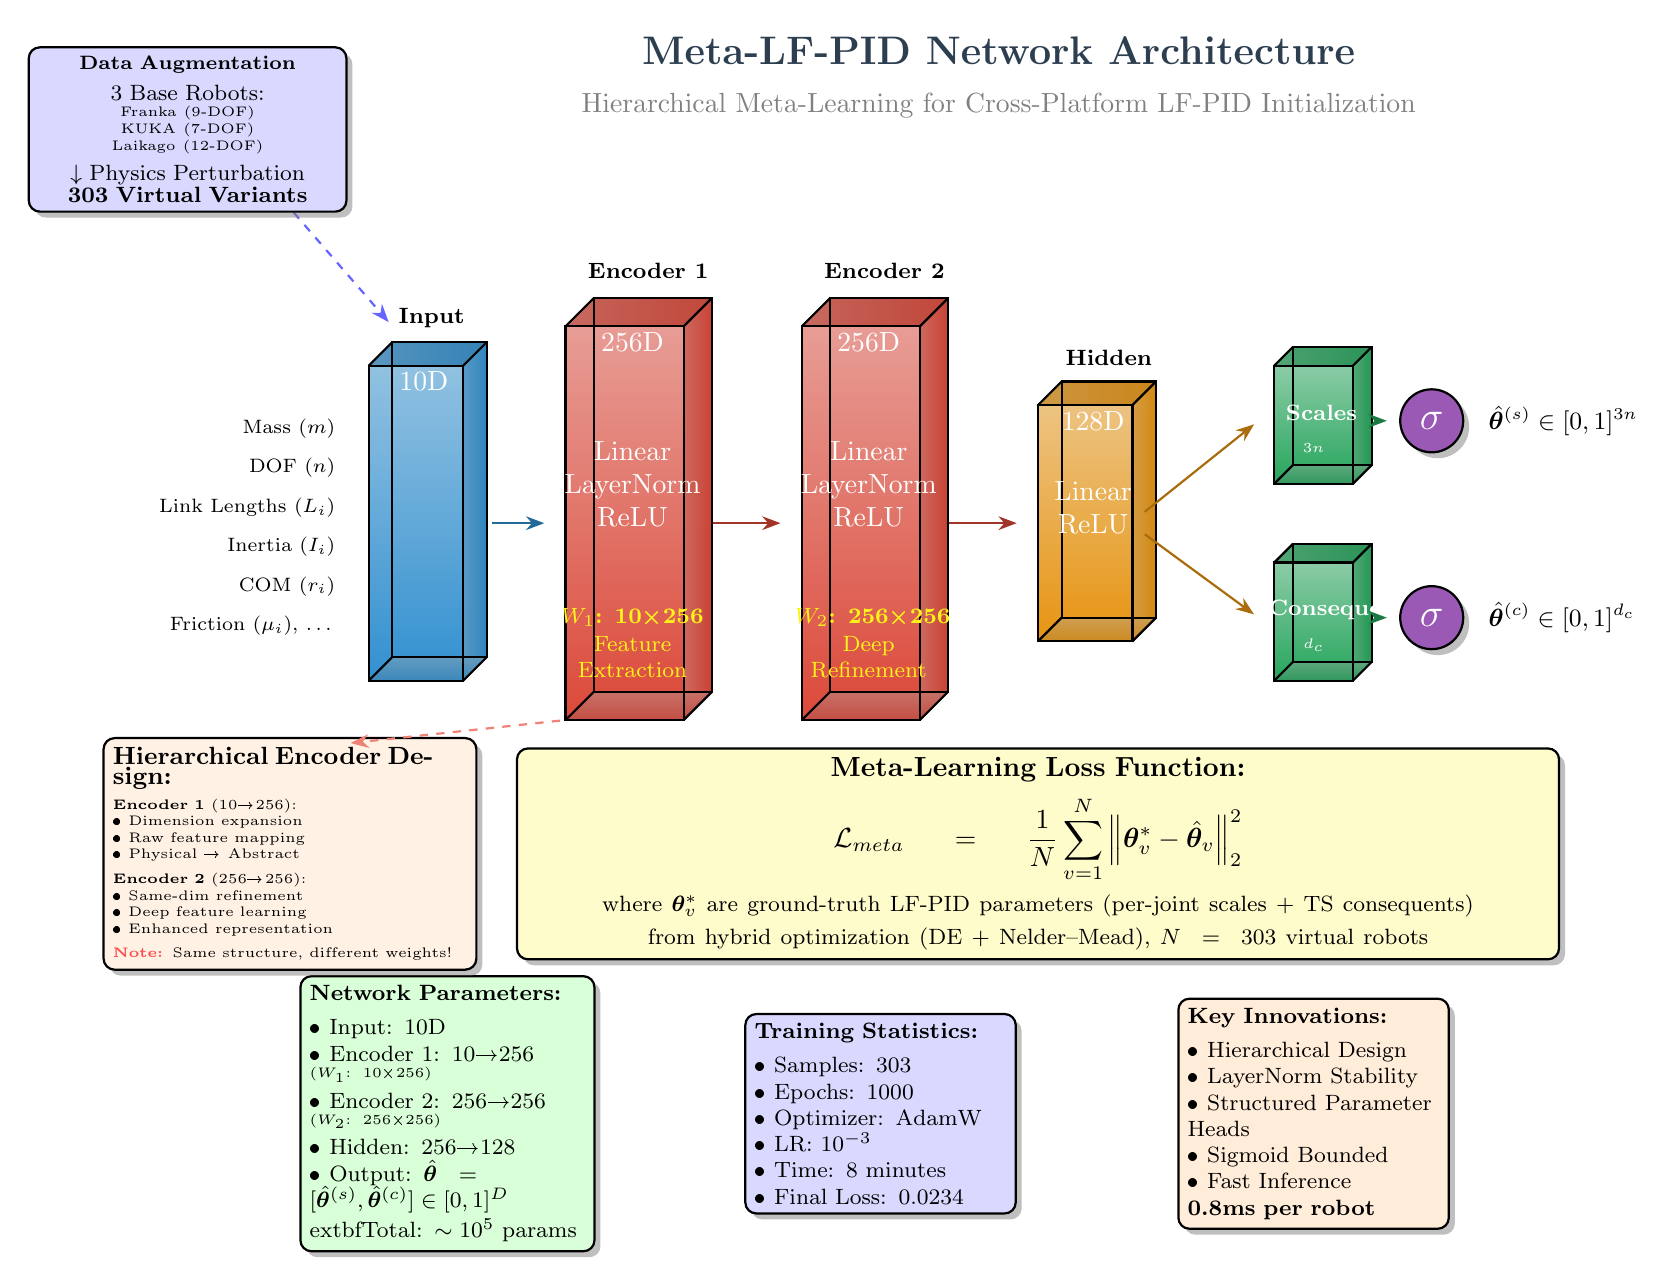
\begin{tikzpicture}[
    font=\rmfamily\small,
    >=Stealth,
    node distance=0.5cm,
    layer/.style={rectangle, draw=black, thick, minimum width=1.5cm, minimum height=3cm, fill=#1, drop shadow},
    activation/.style={circle, draw=black, thick, minimum size=0.8cm, fill=#1, drop shadow},
    label/.style={font=\rmfamily\footnotesize\bfseries, text=#1},
    dimension/.style={font=\rmfamily\tiny, text=gray},
    arrow/.style={->, thick, >=Stealth, shorten >=2pt, shorten <=2pt},
    dashedarrow/.style={->, thick, dashed, >=Stealth, shorten >=2pt, shorten <=2pt},
]

%============================================================================
% Title
%============================================================================
\node[font=\rmfamily\Large\bfseries, text=textcolor] at (8, 8) 
    {Meta-LF-PID Network Architecture};
\node[font=\rmfamily\normalsize, text=gray] at (8, 7.3)
    {Hierarchical Meta-Learning for Cross-Platform LF-PID Initialization};

%============================================================================
% Input Layer (10D Robot Features)
%============================================================================
\drawcube{0}{0}{1.2}{4}{1}{inputcolor}
\node[label=black] at (0.8, 4.6) {\textbf{Input}};
\node[text=white,font=\rmfamily\normalsize] at (0.7, 3.8) {10D};

% 输入特征标注(左侧 - 加大字体)
\node[anchor=east, font=\rmfamily\scriptsize, text width=2.5cm, align=right] at (-0.3, 3.2) 
    {Mass ($m$)};
\node[anchor=east, font=\rmfamily\scriptsize, text width=2.5cm, align=right] at (-0.3, 2.7) 
    {DOF ($n$)};
\node[anchor=east, font=\rmfamily\scriptsize, text width=2.5cm, align=right] at (-0.3, 2.2) 
    {Link Lengths ($L_i$)};
\node[anchor=east, font=\rmfamily\scriptsize, text width=2.5cm, align=right] at (-0.3, 1.7) 
    {Inertia ($I_i$)};
\node[anchor=east, font=\rmfamily\scriptsize, text width=2.5cm, align=right] at (-0.3, 1.2) 
    {COM ($r_i$)};
\node[anchor=east, font=\rmfamily\scriptsize, text width=2.5cm, align=right] at (-0.3, 0.7) 
    {Friction ($\mu_i$), \dots};

%============================================================================
% Encoder Layer 1 (256D)
%============================================================================
\drawcube{2.5}{-0.5}{1.5}{5}{1.2}{encodercolor}
\node[label=black] at (3.55, 5.2) {\textbf{Encoder 1}};
\node[text=white,font=\rmfamily\normalsize] at (3.35, 4.3) {256D};

% Linear + LayerNorm + ReLU
\node[font=\rmfamily\normalsize, text=white, align=center] at (3.35, 2.5) 
    {Linear\\LayerNorm\\ReLU};

% 权重矩阵标注
\node[font=\rmfamily\footnotesize, text=yellow!90, align=center] at (3.35, 0.8)
    {\textbf{$W_1$: 10×256}};

% 功能标注
\node[font=\rmfamily\footnotesize, text=yellow!90, align=center] at (3.35, 0.3)
    {Feature\\Extraction};

% 连接箭头
\draw[arrow, inputcolor!70!black] (1.5, 2) -- (2.3, 2);

% Dropout标注
\node[fill=gray, opacity=0.7, rounded corners, text=white, font=\tiny] 
    at (3.25, -1.2) {Dropout 0.1};

%============================================================================
% Encoder Layer 2 (256D)
%============================================================================
\drawcube{5.5}{-0.5}{1.5}{5}{1.2}{encodercolor}
\node[label=black] at (6.55, 5.2) {\textbf{Encoder 2}};
\node[text=white,font=\rmfamily\normalsize] at (6.35, 4.3) {256D};

\node[font=\rmfamily\normalsize, text=white, align=center] at (6.35, 2.5)
    {Linear\\LayerNorm\\ReLU};

% 权重矩阵标注(与Encoder 1不同)
\node[font=\rmfamily\footnotesize, text=yellow!90, align=center] at (6.40, 0.8)
    {\textbf{$W_2$: 256×256}};

% 功能标注
\node[font=\rmfamily\footnotesize, text=yellow!90, align=center] at (6.35, 0.3)
    {Deep\\Refinement};

% 连接箭头
\draw[arrow, encodercolor!70!black] (4.3, 2) -- (5.3, 2);

\node[fill=gray, opacity=0.7, rounded corners, text=white, font=\tiny]
    at (6.25, -1.2) {Dropout 0.1};

%============================================================================
% Hidden Layer (128D)
%============================================================================
\drawcube{8.5}{0.5}{1.2}{3}{1}{hiddencolor}
\node[label=black] at (9.4, 4.1) {\textbf{Hidden}};
\node[text=white,font=\rmfamily\normalsize] at (9.2, 3.3) {128D};

\node[font=\rmfamily\normalsize, text=white, align=center] at (9.2, 2.2)
    {Linear\\ReLU};

% 连接箭头
\draw[arrow, encodercolor!70!black] (7.3, 2) -- (8.3, 2);

%============================================================================
% Output Heads (2个并行输出:只学习尺度因子与TS后件)
%============================================================================

% Scaling head (per-joint input scaling factors)
\drawcube{11.5}{2.5}{1}{1.5}{0.8}{outputcolor}
\node[label=white, font=\rmfamily\footnotesize\bfseries] at (12.1, 3.4) {Scales};
\node[dimension, text=white] at (12, 2.95) {$3n$};

% TS consequent head (per-joint TS consequents)
\drawcube{11.5}{0.0}{1}{1.5}{0.8}{outputcolor}
\node[label=white, font=\rmfamily\footnotesize\bfseries] at (12.1, 0.9) {TS Consequents};
\node[dimension, text=white] at (12, 0.45) {$d_c$};

% 从Hidden到两个Head的连接
\draw[arrow, hiddencolor!70!black] (9.8, 2.1) -- (11.3, 3.3);
\draw[arrow, hiddencolor!70!black] (9.8, 1.9) -- (11.3, 0.8);

%============================================================================
% Sigmoid激活函数
%============================================================================
\node[activation=activationcolor, font=\Large, text=white] at (13.5, 3.3) {$\sigma$};
\node[activation=activationcolor, font=\Large, text=white] at (13.5, 0.8) {$\sigma$};

% 连接
\draw[arrow, outputcolor!70!black] (12.7, 3.3) -- (13, 3.3);
\draw[arrow, outputcolor!70!black] (12.7, 0.8) -- (13, 0.8);

%============================================================================
% 最终输出标注(参数向量输出)
%============================================================================
\node[anchor=west, font=\rmfamily\small] at (14.1, 3.3)
    {$\hat{\bm{\theta}}^{(s)} \in [0,1]^{3n}$};
\node[anchor=west, font=\rmfamily\small] at (14.1, 0.8)
    {$\hat{\bm{\theta}}^{(c)} \in [0,1]^{d_c}$};

%============================================================================
% 底部:损失函数和训练信息
%============================================================================
\node[draw, thick, rounded corners, fill=yellow!20, text width=13cm, align=center,
      font=\rmfamily\normalsize, drop shadow] at (8.5, -2.2)
{
    \textbf{Meta-Learning Loss Function:}\\[0.15cm]
    $\displaystyle \mathcal{L}_{meta} = \frac{1}{N}\sum_{v=1}^{N} \left\|\bm{\theta}_v^* - \hat{\bm{\theta}}_v\right\|_2^2$\\[0.12cm]
    \footnotesize where $\bm{\theta}_v^*$ are ground-truth LF-PID parameters (per-joint scales + TS consequents)\\
    \footnotesize from hybrid optimization (DE + Nelder--Mead), $N=303$ virtual robots
};

%============================================================================
% 底部信息框 - 三个并排(增加间距)
%============================================================================

% 左侧:网络参数
\node[draw, thick, rounded corners, fill=green!15, text width=3.5cm, align=left,
      font=\rmfamily\footnotesize, drop shadow] at (1, -5.5)
{
    \textbf{Network Parameters:}\\[0.1cm]
    • Input: 10D\\
    • Encoder 1: 10→256\\
    \tiny   ($W_1$: 10×256)\\[0.05cm]
    \footnotesize • Encoder 2: 256→256\\
    \tiny   ($W_2$: 256×256)\\[0.05cm]
    \footnotesize • Hidden: 256→128\\
    • Output: $\hat{\bm{\theta}}=[\hat{\bm{\theta}}^{(s)},\hat{\bm{\theta}}^{(c)}] \in [0,1]^D$\\[0.05cm]
    	extbf{Total: $\sim 10^5$ params}
};

% 中间:训练统计
\node[draw, thick, rounded corners, fill=blue!15, text width=3.2cm, align=left,
      font=\rmfamily\footnotesize, drop shadow] at (6.5, -5.5)
{
    \textbf{Training Statistics:}\\[0.1cm]
    • Samples: 303\\
    • Epochs: 1000\\
    • Optimizer: AdamW\\
    • LR: $10^{-3}$\\
    • Time: 8 minutes\\
    • Final Loss: 0.0234
};

% 右侧:关键创新
\node[draw, thick, rounded corners, fill=orange!15, text width=3.2cm, align=left,
      font=\rmfamily\footnotesize, drop shadow] at (12, -5.5)
{
    \textbf{Key Innovations:}\\[0.1cm]
    • Hierarchical Design\\
    • LayerNorm Stability\\
    • Structured Parameter Heads\\
    • Sigmoid Bounded\\
    • Fast Inference\\
    \textbf{0.8ms per robot}
};

%============================================================================
% 顶部:Data Augmentation来源标注
%============================================================================
\draw[dashedarrow, thick, blue!60] (-1, 6) -- (0.3, 4.5);
\node[draw, thick, rounded corners, fill=blue!15, text width=3.8cm, align=center,
      font=\rmfamily\scriptsize, drop shadow] at (-2.3, 7)
{
    \textbf{Data Augmentation}\\[0.05cm]
    \footnotesize 3 Base Robots:\\
    \tiny Franka (9-DOF)\\
    \tiny KUKA (7-DOF)\\
    \tiny Laikago (12-DOF)\\[0.05cm]
    \footnotesize $\downarrow$ Physics Perturbation\\
    \textbf{303 Virtual Variants}
};

%============================================================================
%============================================================================
% 左下:Encoder设计说明(从右上移到左下)
%============================================================================
\node[draw, thick, rounded corners, fill=orange!10, text width=4.5cm, align=left,
      font=\rmfamily\tiny, drop shadow] (encoder_explanation) at (-1.0, -2.2)
{
    \textbf{\small Hierarchical Encoder Design:}\\[0.1cm]
    \textbf{Encoder 1} (10→256):\\
    • Dimension expansion\\
    • Raw feature mapping\\
    • Physical → Abstract\\[0.1cm]
    \textbf{Encoder 2} (256→256):\\
    • Same-dim refinement\\
    • Deep feature learning\\
    • Enhanced representation\\[0.1cm]
    \textcolor{red!70}{\textbf{Note:}} Same structure, different weights!
};

% 从Encoder 1引出箭头指向说明框
\draw[dashedarrow, thick, encodercolor!70] (2.5, -0.5) -- (-0.3, -0.8);

\end{tikzpicture}
\end{document}
